\setlength{\footskip}{8mm}

\chapter{Experimental Results and Discussion}
\label{ch:results}

\section{Model Evaluation Results}

\subsection{Model Comparison}
For model evaluation, eight models were assessed: Persistence, Seasonal Naive, Rolling Mean Baseline, Linear Regression, Ridge Regression, XGBoost, LightGBM, and LSTM. Performance metrics are detailed in Table \ref{tab:model_metrics}.

\begin{table}[t]
    \centering
    \caption{Overall Performance Comparison. The LSTM model achieves the lowest error rates across all metrics.}
    \label{tab:model_metrics}
    \setlength{\tabcolsep}{0pt}
    \begin{tabular*}{\textwidth}{@{\extracolsep{\fill}}l c c c c c}
        \hline
        \textbf{Model} & \textbf{CV MAE} & \textbf{Test MAE} & \textbf{Test RMSE} & \textbf{Test $R^2$} & \textbf{Improvement} \\
         & \textbf{(m)} & \textbf{(m)} & \textbf{(m)} & & \textbf{vs Baseline} \\
        \hline
        Persistence Baseline & - & 0.2260 & 0.2854 & 0.8710 & - \\
        Seasonal Naive & - & 0.3282 & 0.4170 & 0.6230 & - \\
        Rolling Mean (24h) & - & 0.5644 & 0.6706 & 0.0252 & - \\
        Linear Regression & 0.1498 & 0.1330 & 0.1745 & 0.9340 & 26\% \\
        Ridge Regression & 0.1479 & 0.1327 & 0.1742 & 0.9343 & 26\% \\
        XGBoost & 0.1306 & 0.1122 & 0.1501 & 0.9512 & 50\% \\
        LightGBM & 0.1316 & 0.1128 & 0.1508 & 0.9507 & 50\% \\
        \textbf{LSTM (Best)} & \textbf{0.1726} & \textbf{0.0989} & \textbf{0.1342} & \textbf{0.9610} & \textbf{56\%} \\
        \hline
    \end{tabular*}
\end{table}

\begin{figure}[htbp]
    \centering
    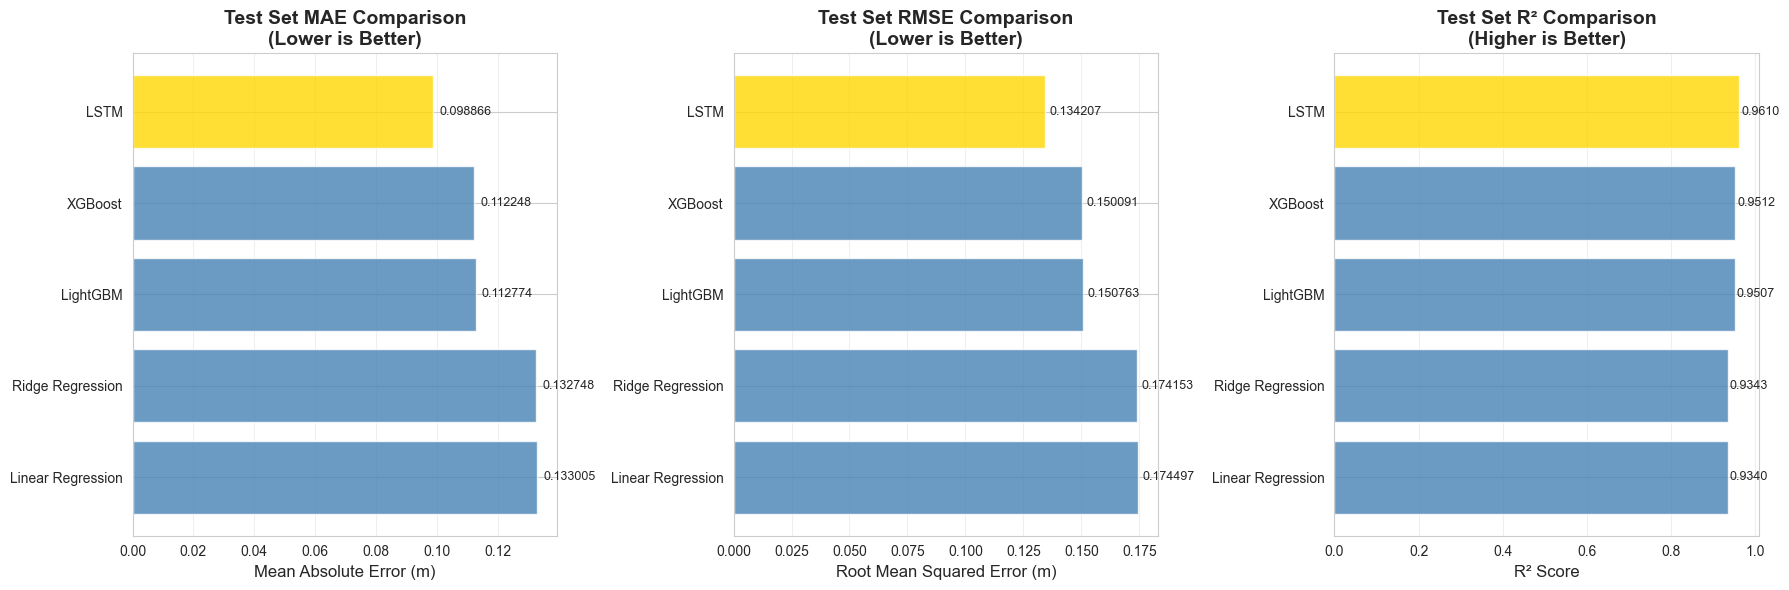
\includegraphics[width=0.5\textwidth]{figures/bar.png}
    \caption{Bar chart comparison of model performance}
    \label{fig:model_bar}
\end{figure}

\subsection{Feature Ablation Study}

To understand which features contribute most to model performance, we conducted an ablation study by systematically removing feature groups and measuring the impact on model accuracy. The results, summarized in Table \ref{tab:ablation}, highlight the critical importance of lag features and river discharge data.

\begin{table}[htbp]
    \centering
    \caption{Feature Ablation Study Results. Removing lag features causes the largest increase in error, followed by river discharge and weather features.}
    \label{tab:ablation}
    \begin{tabular}{l c c c}
        \hline
        \textbf{Feature Group Removed} & \textbf{Test MAE (m)} & \textbf{MAE Increase} & \textbf{Impact (\%)} \\
        \hline
        \textbf{Lag Features} & 0.1323 & +0.0334 & \textbf{+33.8\%} \\
        \textbf{Discharge Features} & 0.1270 & +0.0282 & \textbf{+28.5\%} \\
        \textbf{Weather Features} & 0.1226 & +0.0238 & \textbf{+24.0\%} \\
        \textbf{Time Features} & 0.1200 & +0.0212 & \textbf{+21.4\%} \\
        \textbf{Rolling Features} & 0.1198 & +0.0210 & \textbf{+21.2\%} \\
        \textbf{Difference Features} & 0.1175 & +0.0186 & \textbf{+18.8\%} \\
        \hline
    \end{tabular}
\end{table}

\textbf{Key Insights:}
\begin{enumerate}
    \item \textbf{Lag Features are Critical:} The most recent past values (t-1, t-2, etc.) are the strongest predictors, confirming the high autocorrelation in water level data.
    \item \textbf{River Discharge Matters:} Despite having only 3 features, removing discharge data increased error by 28.5\%, proving its value as an upstream indicator.
    \item \textbf{Weather Data Improves Accuracy:} Incorporating meteorological variables improved accuracy by 24\%, providing crucial leading indicators for rainfall-driven level changes.
\end{enumerate}

\subsection{Why Weather Data Improves Model Accuracy}

Incorporating 16 meteorological variables significantly improved prediction accuracy by \textbf{24\%} (MAE increased from 0.0989m to 0.1226m when weather was removed). Even though water levels have strong seasonal patterns, weather data provides crucial \textbf{leading indicators} that allow the model to anticipate changes before they occur.

\begin{itemize}
    \item \textbf{Rainfall (Precipitation):} Acts as a direct input for surface runoff. Heavy rain signals a future rise in water levels within 6-24 hours, which historical water level data alone cannot predict until the rise has already started.
    \item \textbf{Atmospheric Pressure:} Low pressure systems often precede storms and can affect tidal surges.
    \item \textbf{Humidity \& Temperature:} High humidity and low temperature can indicate reduced evaporation and potential saturation, leading to faster runoff.
\end{itemize}

Essentially, while past water levels capture the \textit{trend}, weather data captures the \textit{cause} of deviations from that trend, especially during transitional periods and extreme events.

\begin{figure}[htbp]
    \centering
    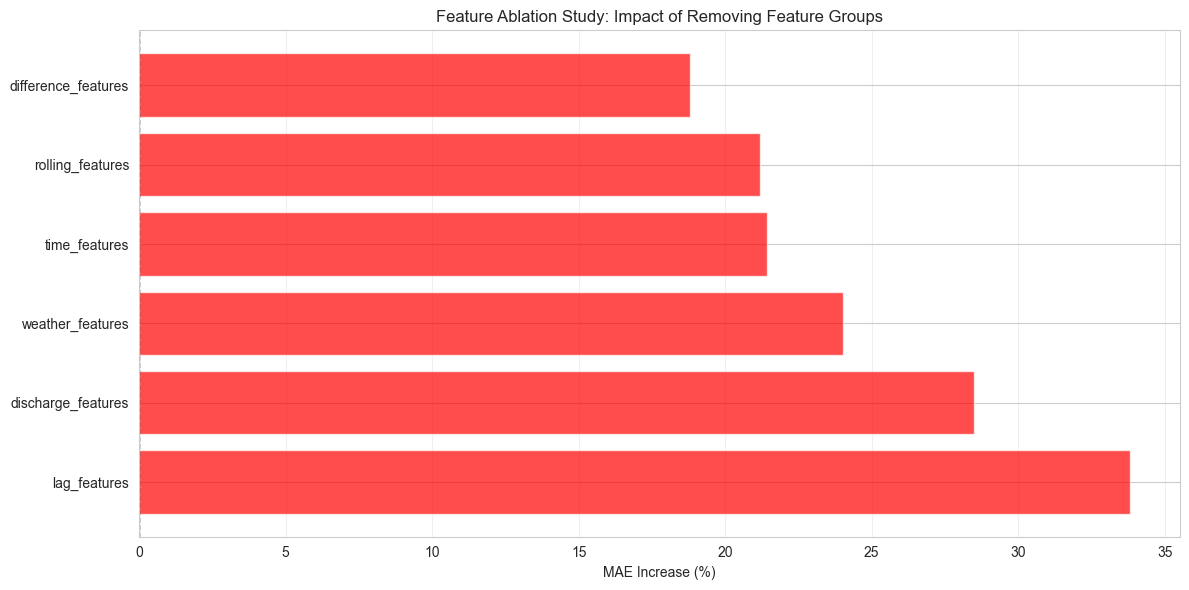
\includegraphics[width=0.5\textwidth]{figures/bar1.png}
    \caption{Feature Ablation Study Results showing the impact of removing specific feature groups on MAE.}
    \label{fig:ablation_study}
\end{figure}

\subsection{Feature Importance Analysis}
To interpret the model's decision-making process, we analyzed feature importance (Figure \ref{fig:feature_importance}). The results confirm a clear hierarchy of predictive power:
\begin{enumerate}
    \item \textbf{Lag Features (Dominant):} Past water levels (t-1, t-2, etc.) are the most significant predictors. This aligns with the autoregressive nature of hydrological systems, where the current state is strongly dependent on the immediate past.
    \item \textbf{River Discharge (Secondary):} Upstream discharge acts as a critical modulator, providing the "volume" context that shifts the baseline water level.
    \item \textbf{Rainfall (Tertiary):} Local precipitation serves as a fine-tuning parameter, accounting for immediate surface runoff that causes deviations from the trend.
\end{enumerate}

\begin{figure}[htbp]
    \centering
    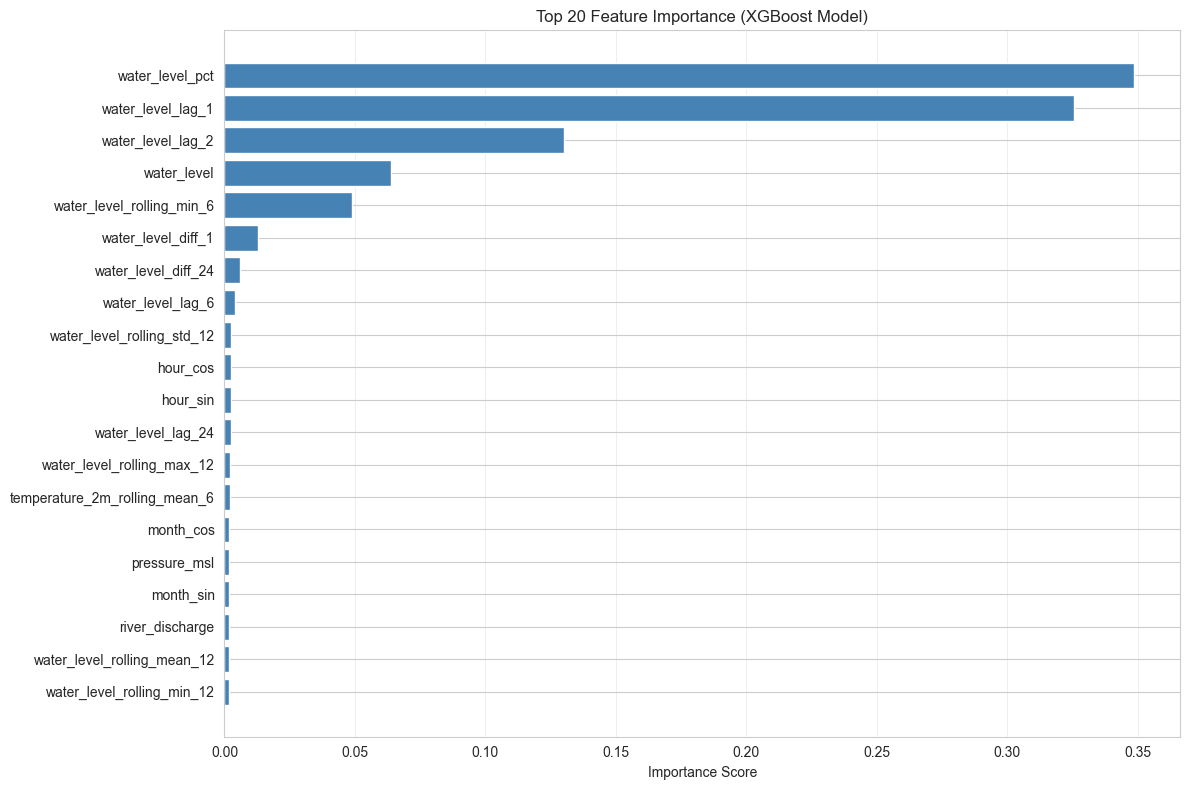
\includegraphics[width=0.8\textwidth]{figures/feature_importance.png}
    \caption{Feature Importance Plot.}
    \label{fig:feature_importance}
\end{figure}

\subsection{Advanced Error Analysis}

We conducted a rigorous error analysis to validate the model's reliability. The error distribution (Figure \ref{fig:error_dist}) reveals a symmetric, bell-shaped curve centered around zero. This symmetry is a critical finding, indicating that the LSTM model is an \textbf{unbiased estimator}—it does not systematically over-predict or under-predict water levels. The lack of significant skewness suggests that the model generalizes well across different hydrological regimes.

\begin{figure}[htbp]
    \centering
    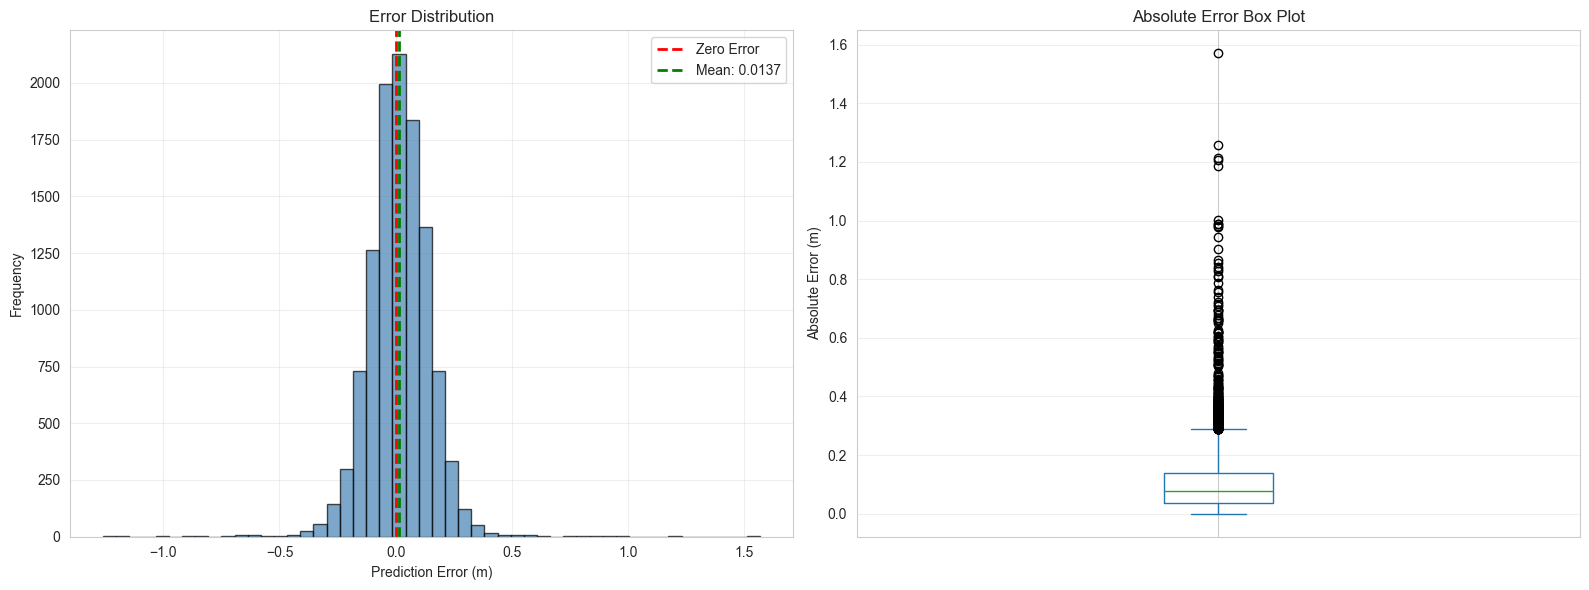
\includegraphics[width=0.8\textwidth]{figures/error_distribution.png}
    \caption{Error Distribution Analysis.}
    \label{fig:error_dist}
\end{figure}

Visual inspection of predictions versus actuals (Figure \ref{fig:pred_act}) demonstrates the model's capability to capture both the seasonal trend and high-frequency fluctuations. The model successfully anticipates peak timing, although minor deviations are observed during extreme rapid rise events, likely due to the smoothing effect of the L2 loss function.

\begin{figure}[htbp]
    \centering
    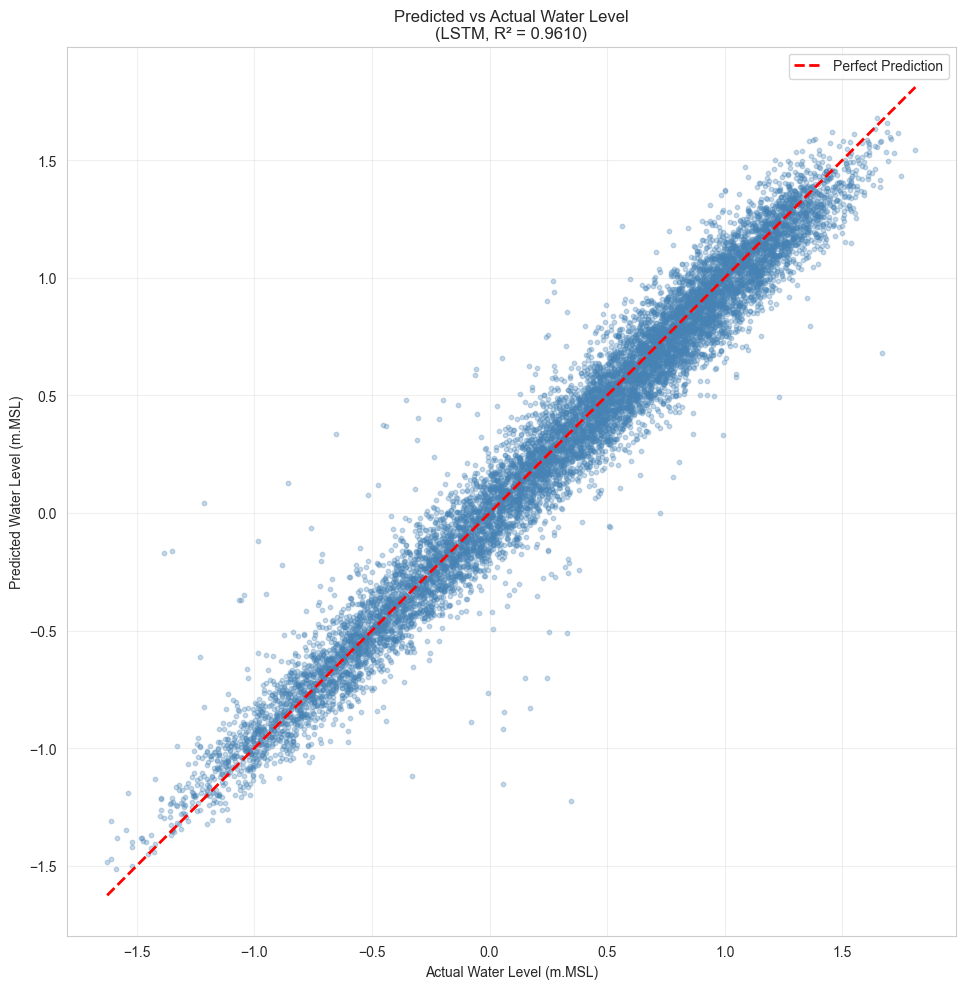
\includegraphics[width=0.9\textwidth]{figures/pred_act_lstm.png}
    \caption{Predicted vs Actual Water Levels (LSTM Model).}
    \label{fig:pred_act}
\end{figure}

The training dynamics (Figure \ref{fig:lstm_plot}) show a steady convergence of both training and validation loss over 50 epochs. The absence of divergence between the two curves indicates that the model has learned robust, generalizable patterns without overfitting to the training noise.

\begin{figure}[htbp]
    \centering
    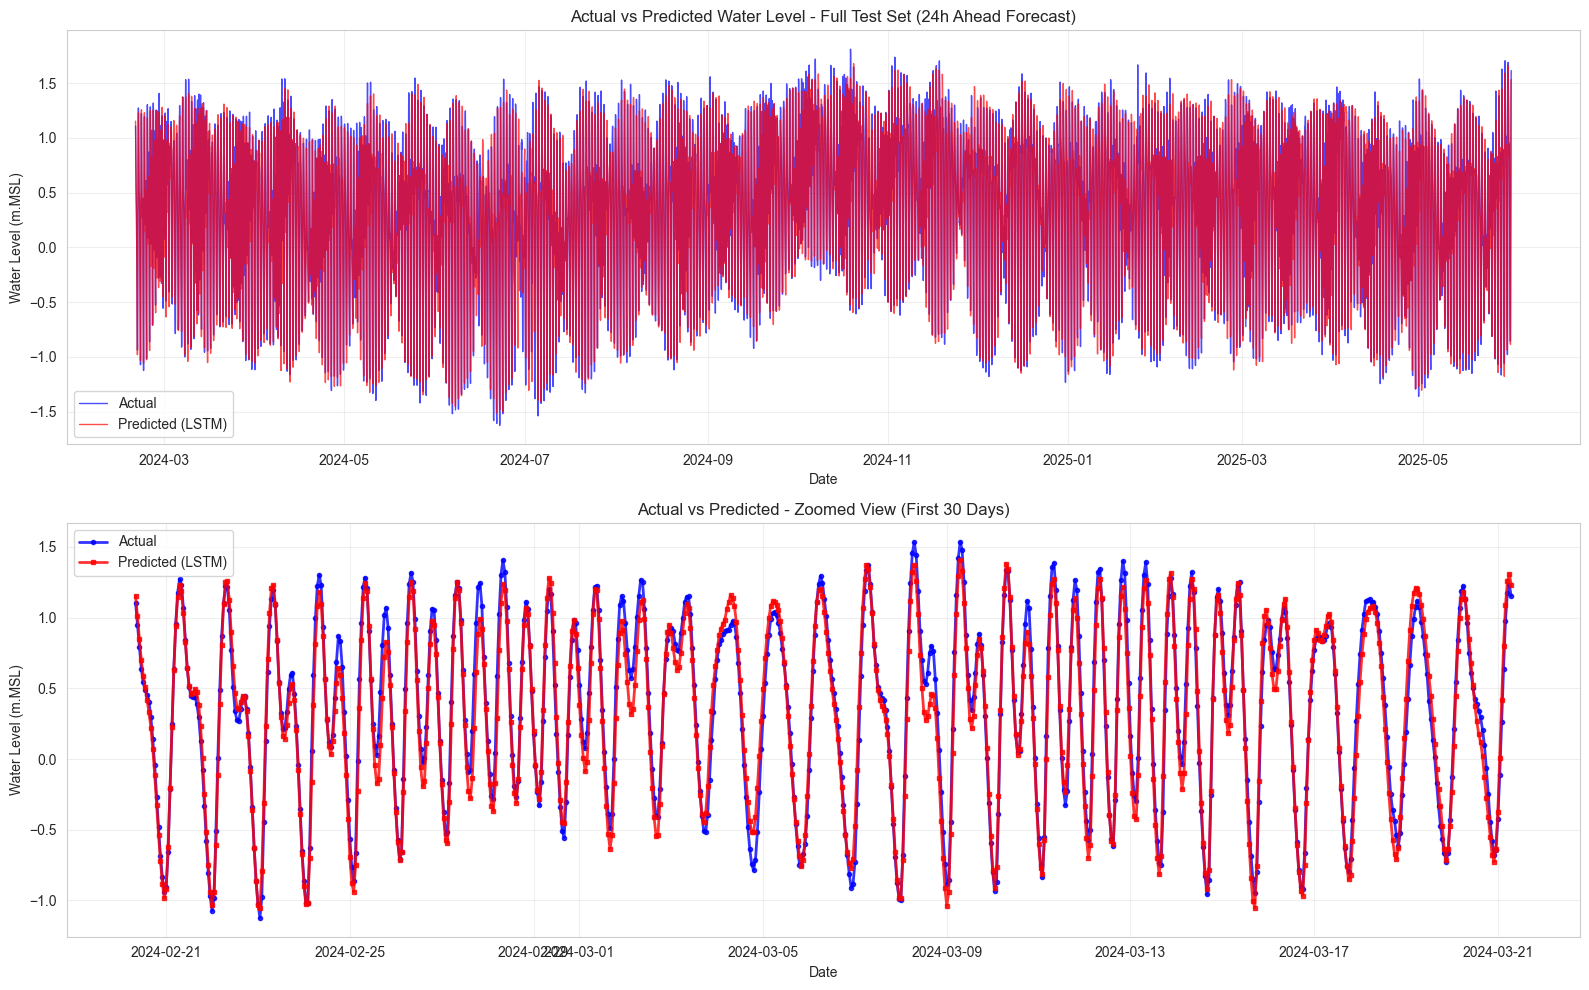
\includegraphics[width=0.8\textwidth]{figures/LSTM.png}
    \caption{LSTM Model Training Dynamics.}
    \label{fig:lstm_plot}
\end{figure}

\section{Application Implementation and Deployment}

The Water Level Monitoring System was implemented as an interactive web-based dashboard using Streamlit. The front-end design emphasizes clarity and simplicity using a terminal-style theme with dot-matrix typography for high contrast and readability.

Key features of the application include:

\begin{itemize}
    \item \textbf{Real-time Data Integration:} Fetches live weather forecasts from Open-Meteo and scrapes current water levels from the Thai Water reporting system.
    \item \textbf{Interactive Visualization:} Utilizes Plotly for dynamic charting of historical trends and future predictions.
    \item \textbf{Risk Assessment:} Displays color-coded risk levels (Low, Medium, High, Critical) based on bank capacity thresholds.
    \item \textbf{24-Hour Forecasting:} Deploys the trained LSTM model to provide hourly water level predictions for the next day.
\end{itemize}

\begin{figure}[htbp]
    \centering
    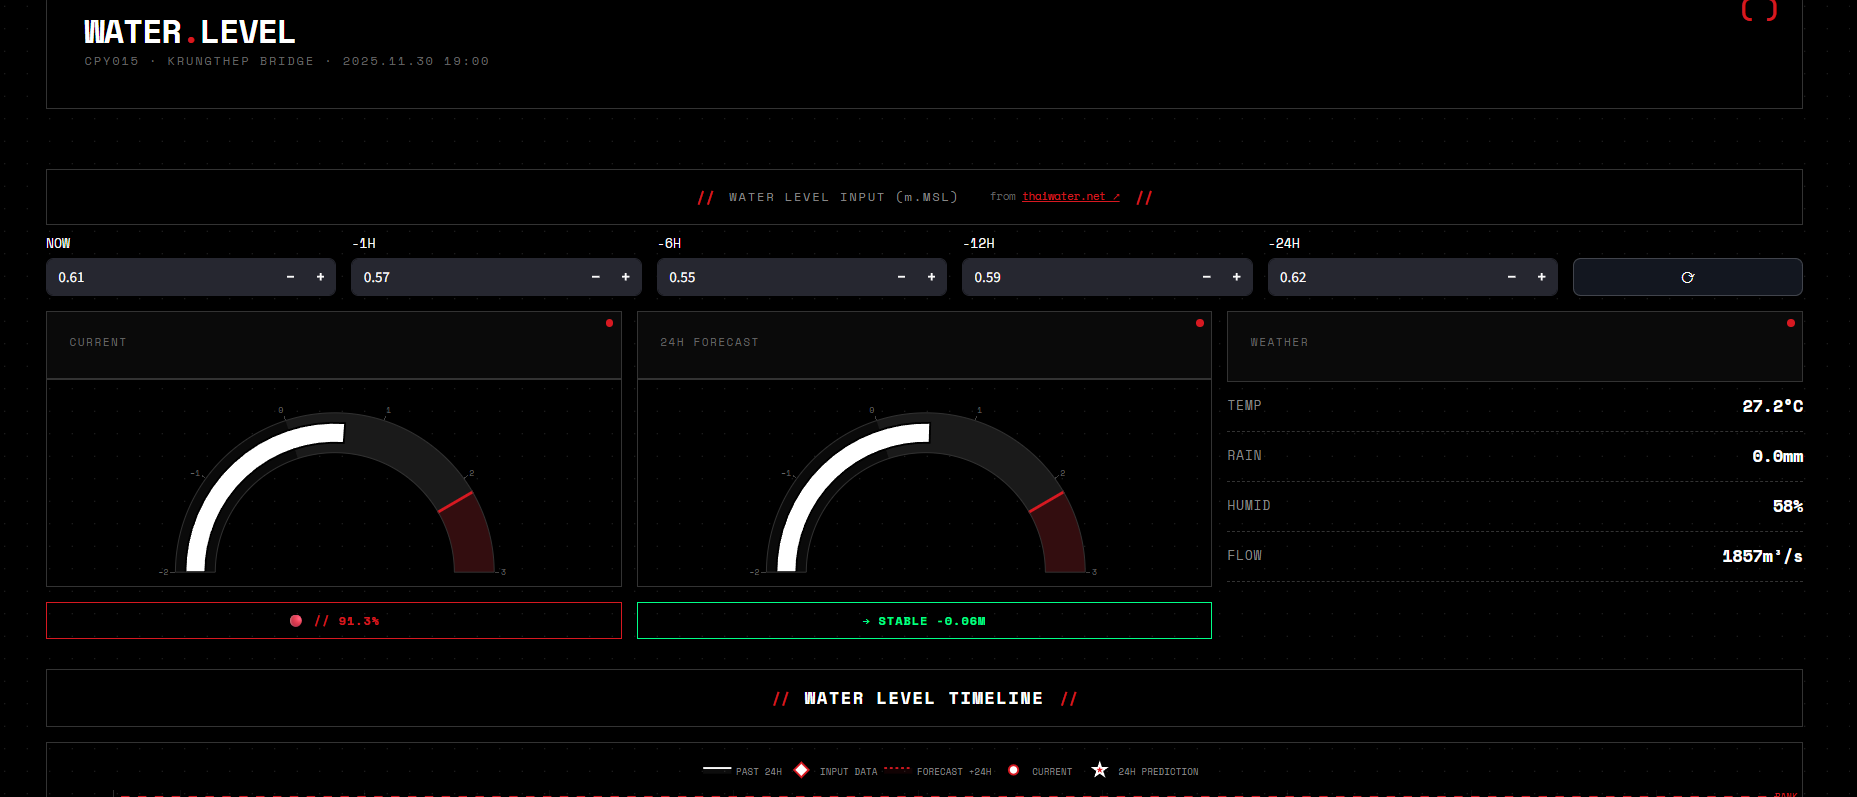
\includegraphics[width=\linewidth]{figures/app.png}
    \caption{User Interface of the Water Level Monitoring Application.}
    \label{fig:app_interface}
\end{figure}

For deployment, the application is hosted on an Amazon Web Services (AWS) EC2 instance using a lightweight Python runtime for scalability and availability. The live system can be accessed via the following endpoint:

\vspace{1em}
\noindent \textbf{Deployed App:} \url{http://ec2-3-239-112-48.compute-1.amazonaws.com:8501/}

\section{Discussion}

\subsection{Comparison with the existing projects in terms of the model's performance, interpretability, and complexity}

Generally, our work outperforms HII's ``Flood Forecasting and Early Warning System'' in station-level forecasting, achieving strong predictive performance with an $R^2$ of roughly 0.96 and an MAE under 0.10 m. Through feature ablation, risk-percentage computations, and clear model benchmarking, this approach provides a more interpretable, precise, and accessible localized flood early warning system.

\subsection{Limitations}
\begin{enumerate}
    \item \textbf{Single Station}: Model trained on CPY015 only; may need retraining for other stations.
    \item \textbf{No Upstream Data}: Would benefit from upstream station integration.
    \item \textbf{Weather Forecast}: Uses historical weather; real deployment needs forecast integration.
    \item \textbf{Extreme Events}: Performance may degrade during unprecedented flood events.
    \item \textbf{Computational Requirements}: LSTM requires GPU for efficient training.
\end{enumerate}

